\chapter{Statistics: Sampling}\label{Statistics: Sampling}

\begin{figure}[h]
    \centering
    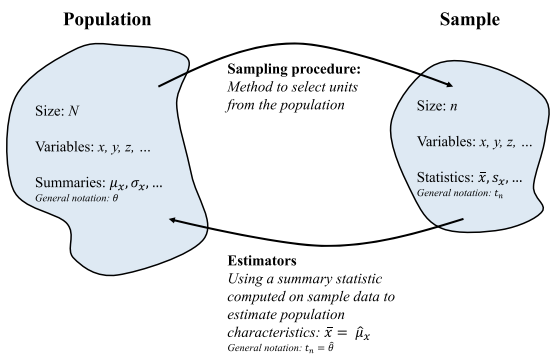
\includegraphics[width=\linewidth, height=4cm, keepaspectratio]{Pictures/statistics/population-and-sample.png}
\end{figure}

\begin{table}[h]
    \centering
    \begin{tabular}{|l|c|c|}
        \hline

        & \textbf{Population} & \textbf{Sample}\\
        \hline

        \textbf{Size} & $N$ & $n$ \\
        \hline

        \textbf{Variables} & $x,y,z,\cdots$ & $x,y,z,\cdots$ \\
        \hline

        \textbf{Summaries/ Statistics} & $\mu_x,\sigma_x,\cdots$ & $\bar{x}, s_x, \cdots$\\
        \hline

        \textbf{General Notation} & $\theta$ & $t_n$\\
        \hline
    \end{tabular}
\end{table}


\section{Convenience Sampling \cite{ism-1}} \label{Convenience Sampling}

\begin{enumerate}
    \item collects only units from the population that can be \textbf{easily obtained}

    \item may provide a \textbf{biased} sample

    \item often justified by using the argument of \textbf{population homogeneity}
\end{enumerate}

\section{Haphazard Sampling \cite{ism-1}}
\label{Haphazard Sampling}

\begin{enumerate}
    \item Despite the feeling of randomness when performing haphazard sampling, often the resulting sample is not truly random.

\end{enumerate}


\section{Purposive Sampling \cite{ism-1}}\label{Purposive Sampling}

\begin{enumerate}
    \item tries to sample units for a specific purpose. 

    \item This means that the collection of units is focused on one or more particular characteristics and hence it implies that only units that are more alike are sampled.
\end{enumerate}


\section{Simple Random Sampling \cite{ism-1}}\label{Simple Random Sampling}

\renewcommand{\arraystretch}{2.5}
\begin{longtable}{|p{5cm}|p{9cm}|}
    \hline\endfirsthead
    \hline\endhead
    \hline\endfoot
    \hline\endlastfoot

    \textbf{Number of possible samples} & \( \dfrac{N!}{n!(N-n)!} \) \\
    \hline

    \textbf{Probability that $S_k$ is selected} & $\pi_k = \dfrac{1}{K}$ \\
    \hline

    \textbf{Probability that a specific unit is part of the sample} & $\dfrac{n}{N}$ \\
    \hline

    \textbf{Mean ($\mathbb{E}(T)$)} & $
        \mathbb{E}(T) = 
        \dfrac{1}{K} \displaystyle\sum_{k=1}^{K}
        \bar{x}_k 
        =
        \dfrac{1}{nK} \displaystyle\sum_{k=1}^{K}
        \displaystyle\sum_{i \in S_k} x_i
        =
        \dfrac{1}{N} \displaystyle\sum_{i=1}^{N} x_i
        = \mu
    $ \\[2ex]
    \hline

    \textbf{Estimator of Mean ($\bar{x}_k$)} & $
        \bar{x}_k=
        \dfrac{1}{n} \displaystyle\sum_{i=1}^{n} x_i
    $ \\[2ex]
    \hline

    \textbf{Bias} & $
        bias(c\bar{x}_k) = (c-1)\mu
        \quad\quad\quad
        bias(\bar{x}_k) = 0
    $ \\[1ex]
    \hline

    \textbf{MSE ($MSE(c\bar{x}_k)$)} & $
        MSE(c\bar{x}_k) 
        = [(c-1)\mu]^2 +
        c^2 \sigma^2 \left(\dfrac{N}{N-1} \right)\left( 1-\dfrac{n}{N} \right)\dfrac{1}{n}
    $\\[1ex]
    & $MSE(\bar{x}_k) 
        = \sigma^2 \left(\dfrac{N}{N-1} \right)\left( 1-\dfrac{n}{N} \right)\dfrac{1}{n}$ \\[1ex]
    \hline

    \textbf{Estimator of MSE ($\hat{MSE}(\bar{x}_k)$)} & $
        \hat{MSE}(\bar{x}_k) = \left(\dfrac{N-n}{Nn} \right)s_k^2
    $\\[1ex]
    \hline

    \textbf{Variance ($\sigma^2$)} & $
        \sigma^2 = \dfrac{1}{N} \displaystyle\sum_{i=1}^{N}
        (x_i - \mu)^2
    $\\[1ex]
    \hline

    \textbf{Estimator of Variance ($s_k^2$)} & $
        s_k^2 = \left(\dfrac{1}{n-1}\right) \displaystyle\sum_{i\in S_k}
        (x_i - \bar{x}_k)^2
    $\\[1ex]
    \hline

    \textbf{SE ($SE(c\bar{x}_k)$)} & $
        SE(c\bar{x}_k) = \sqrt{
            c^2 \sigma^2 \left(\dfrac{N}{N-1} \right)\left( 1-\dfrac{n}{N} \right)\dfrac{1}{n}
        }
    $\\[1ex]
    \hline
\end{longtable}

\section{Systematic Sampling \cite{ism-1}}\label{Systematic Sampling}

\begin{enumerate}
    \item Population should be divided into $n$ groups and the order of the units (if some order exists) should be maintained (or otherwise fix the order).

    \item each group consists of $m$ units (thus the population size is $N = nm$) \textbf{ordered} from $1$ to $m$ in each group.
    \[
        m \in \{1,2,\cdots,N\}
    \]

    \item from each of the $n$ groups the $k$th unit is collected, forming the sample of $n$ units. 
    \[
        S_k = \{ k, k+m,k+2m,\cdots,k+(n-1)m \}
        \hfill
        (k \in \{1,2,\cdots,m\})
    \]
\end{enumerate}

\begin{longtable}{|p{5cm}|p{9cm}|}
    \hline\endfirsthead
    \hline\endhead
    \hline\endfoot
    \hline\endlastfoot

    \textbf{Probability of selecting $S_k$} & $\dfrac{1}{m}$\\[1ex]
    \hline

    \textbf{Mean ($\mu$)} & $
        \mu = \dfrac{1}{N}
        \displaystyle\sum_{h=1}^{m}
        \displaystyle\sum_{i=1}^{n} 
        x_{h+m(i-1)}
    $\\[1ex]
    \hline

    \textbf{Estimator of Mean ($\bar{x}_k$)} & $
        \bar{x}_k = 
        \dfrac{1}{n} \displaystyle\sum_{i=1}^{n}
        x_{h+m(i-1)}
    $\\[1ex]
    \hline

    \textbf{Variance ($\sigma^2$)} & $
        \sigma^2 = 
        \dfrac{1}{N}
        \displaystyle\sum_{k=1}^{m}
        \displaystyle\sum_{i=1}^{n}
        (x_{k+m(i-1)} - \mu)^2
    $\\[1ex]
    \hline

    \textbf{Estimator of Variance ($s_k^2$)} & $
        s_k^2 = \left(\dfrac{1}{n-1}\right)
        \displaystyle\sum_{i=1}^{n}
        (x_{k+m(i-1)} - \bar{x}_k)^2
    $\\[1ex]
    \hline

    \textbf{Bias} & $bias(\bar{x}_k) = 0$\\
    \hline

    \textbf{MSE} & $
        MSE = \sigma^2 -
        \dfrac{1}{N}
        \displaystyle\sum_{h=1}^{m}
        \displaystyle\sum_{i=1}^{n}
        (x_{h+m(i-1)} - \bar{x}_h)^2
    $\\[1ex]
    \hline
\end{longtable}


\section{Stratified Sampling \cite{ism-1}}\label{Stratified Sampling}

\begin{enumerate}
    \item numbers of units across the \textbf{subpopulations} $S_h$ (called \textbf{strata}\indexlabel{strata}) are (substantially) different $N_h$

    \item selecting the same fraction/ proportion of the units from each stratum we are certain that each stratum is included in the sample, and represents the population

    \item If the ratio of the sample size $n_h$ and stratum size $N_h$ is the same across all strata, each unit in the population has the same probability of being collected in the sample. This type of stratified sampling is called \textbf{proportional stratified sampling}\indexlabel{proportional stratified sampling}.

    \item[] $S_h = \{ S_{h,1}, S_{h,2},\cdots, S_{h,N_h} \}$

    \item[] $K_h = \dfrac{N_h!}{n_h!(N_h-n_h)!}$

    \item[] $w_h = \dfrac{N_h}{N}$

    \item[] $
        K_S = 
        \dfrac{N_1!}{n_1!(N_1-n_1)!} 
        \times
        \dfrac{N_1!}{n_1!(N_1-n_1)!} 
        \times
        \cdots
        \times
        \dfrac{N_M!}{n_M!(N_M-n_M)!}
        =
        \displaystyle\prod_{M}^{i=1} \dfrac{N_i!}{ni!(N_i-n_i)!}
    $

    \item[] $
        \displaystyle\sum_{i=1}^{M} N_i = N
        \quad\quad
        \displaystyle\sum_{i=1}^{M} n_i = n
    $


\end{enumerate}

\begin{longtable}{|p{5cm}|p{9cm}|}
    \hline\endfirsthead
    \hline\endhead
    \hline\endfoot
    \hline\endlastfoot

    number of possible samples that can be collected with stratified random sampling & $K_S$\\
    \hline

    \textbf{Mean ($\mu_h$)} & $
        \mu_h = \dfrac{1}{N_h} 
        \displaystyle\sum_{i=1}^{N_h} x_{hi}
    $\\[1ex]
    \hline

    \textbf{Estimator of Mean ($\bar{x}_{h,k}$)} & $
        \bar{x}_{h,k} = \dfrac{1}{n_h} 
        \displaystyle\sum_{i\in S_{h,k}} x_{hi}
    $\\[1ex]
    & $
        \bar{x}_{k} = \displaystyle\sum_{h=1}^{M}
        w_h\bar{x}_{h,k}
        = \displaystyle\sum_{h=1}^{M}
        \left(\dfrac{N_h}{N}\right)
        \left(
            \dfrac{1}{n_h} 
            \displaystyle\sum_{i=1}^{n_h} x_{hi}
        \right)
    $\\[1ex]
    \hline

    \textbf{Variance ($\sigma_h^2$)} & $
        \sigma_h^2=\dfrac{1}{N_h}
        \displaystyle\sum_{i=1}^{N_h}
        (x_{hi} - \mu_{h})^2
    $\\[1ex]
    & \begin{minipage}{5cm}
        $\sigma^2 = \dfrac{1}{N}
        \displaystyle\sum_{h=1}^{M}
        \displaystyle\sum_{i=1}^{N_h}
        (x_{hi}-\mu)^2$ \\
        $=\displaystyle\sum_{h=1}^{M} w_h\sigma_h^2 +
        \displaystyle\sum_{h=1}^{M} w_h(\mu_h - \mu)^2$\\
        (within) \& (between) variances\\
        \vspace{0.1cm}
    \end{minipage}
    \\[2ex]
    \hline

    \textbf{Estimator of Variance ($s_{h,k}^2$)} & $
        s_{h,k}^2 = 
        \dfrac{1}{n_h - 1}
        \displaystyle\sum_{i\in S_{h,k}}
        (x_{hi} - \bar{x}_{h,k})^2
    $\\
    \hline

    \textbf{Bias} & 0\\
    \hline

    \textbf{MSE} & $
        MSE = \displaystyle\sum_{h=1}^{M}
        \left[
            \left(
                \dfrac{N_h^2(N_h-n_h)}{n_h(N_h-1)N^2}
            \right)
            \sigma_h^2
        \right]
    $\\[1ex]
    & $
        MSE(\bar{x}_k) = \displaystyle\sum_{h=1}^{M}
        w_h^2 MSE(\bar{x}_{h,k})
        = \displaystyle\sum_{h=1}^{M}
        \dfrac{N_h(1-f_h)w_h^2\sigma_h^2}{(N_h-1)n_h}
    $\\[1ex]
    \hline

    \textbf{Estimator of MSE ($\hat{MSE}$)} & $
        \hat{MSE}(\bar{x}_k) = \dfrac{1}{n_h}
        \displaystyle\sum_{h=1}^{M}
        (1-f_h)w_h^2 s_{h,k}^2
    $\\[1ex]
    \hline

    \textbf{SE} & $
        SE(cT) = c\cdot SE(T)
    $\\[1ex]
    \hline
    
    \textbf{Esimator of SE ($\hat{SE}$)} & $
        \hat{SE}(\bar{x}_{h,k}) =
        \sqrt{\dfrac{1-f_h}{n_h}}s_{h,k}
    $\\[1ex]
    \hline
\end{longtable}



\section{Cluster Sampling \cite{ism-1}}\label{Cluster Sampling}

\begin{enumerate}
    \item Directly sampling units from populations is not feasible.

    \item random sampling of groups or clusters of units in the population

    \item Cluster sampling can be less representative than sampling units directly.

    \item cluster sampling introduces a specific structure in the sample which should also be addressed when the data is being analyzed.

    \item The cluster structure introduces two sources of variation in the data being collected.
    \begin{enumerate}
        \item Within-cluster variation
        \item Between-cluster variation
    \end{enumerate}

    \item Cluster sampling is in a way related to stratified sampling
\end{enumerate}

\subsection{Single-stage Cluster Sampling \cite{ism-1}} \label{Single-stage Cluster Sampling}

\begin{enumerate}
    \item uses a random sample of the clusters and then all units from these clusters are selected (aka \textbf{primary cluster units}\indexlabel{primary cluster units})

    \item $x_{hi}$ the value on variable $x$ for unit $i$ in cluster $h$
    \[
        N = \displaystyle\sum_{h=1}^{M} N_h
    \]

    
\end{enumerate}

\begin{longtable}{|p{5cm}|p{9cm}|}
    \hline\endfirsthead
    \hline\endhead
    \hline\endfoot
    \hline\endlastfoot

    \textbf{Mean ($\mu$)} & $
        \mu = \dfrac{1}{N}
        \displaystyle\sum_{h=1}^{M}
        \displaystyle\sum_{i=1}^{N_h}
        x_{hi}
    $\\[1ex]
    \hline

    \textbf{Estimator of Mean} & $
        \bar{x}_h = \mu_h
        \quad\quad
        \bar{x} = \dfrac{1}{m}
        \displaystyle\sum_{h=1}^{m} \bar{x}_h
    $\\[1ex]
    \hline

    
\end{longtable}



























